\documentclass{article}
\usepackage{spconf,amsmath,graphicx}

% Example definitions.
% --------------------
\def\x{{\mathbf x}}
\def\L{{\cal L}}

\title{EE5183 FinTech Final Project Report}

\name{%
  Y.\,N.\ Huang$^{1}$, 
  M.\,C.\ Hsieh$^{1}$, 
  T.\,S.\ Su$^{2}$, 
  M.\,R.\ Yang$^{2}$, 
  H.\,C.\ Tsui$^{2}$, 
  Y.\,T.\ Chen$^{3}$%
  \thanks{All authors contributed equally to this work.}%
}

\address{%
  $^{1}$Graduate Institute of Communication Engineering, National Taiwan University\\
  $^{2}$Graduate Institute of Biomedical Electronics and Bioinformatics, National Taiwan University\\
  $^{3}$Department of Economics, National Taiwan University
}

\begin{document}
%\ninept
%
\maketitle
%
\begin{abstract}
Recommendation systems have long played a critical role in guiding users to relevant content. Prior research focuses primarily on improving accuracy, but concerns about demographic fairness—ensuring equitable treatment across user groups—have become increasingly important. In this paper, we propose a plug-in module that can be seamlessly integrated into any sequential recommendation model to enhance demographic fairness nearly without sacrificing accuracy. Our approach applies a lightweight fairness regularization during training and introduces no additional inference overhead. Experiments on public benchmarks (e.g., MovieLens-1M) show that our method reduces demographic disparity by up to \b{12\%} while maintaining competitive recommendation accuracy. These results demonstrate that fairness can be substantially improved with minimal impact on performance.
\end{abstract}

%
\begin{keywords}
Recommendation System, Demographic, Fairness, Sequential
\end{keywords}
%
\section{Introduction}
\label{sec:intro}
% Paragraph 1: background of recsys
\subsection{Background of Recommendation Systems}
Recommender systems (RS) are indispensable tools for mitigating information overload in domains ranging from e-commerce to streaming media and social platforms \cite{Wang2023FairRecSys}.  Early RS methods—such as collaborative filtering and content‐based filtering—modeled user–item interactions to optimize accuracy metrics like hit rate and RMSE.  In recent years, deep learning techniques, including graph neural networks, have further advanced recommendation quality by capturing complex relational and sequential patterns in user behavior \cite{Dong2022StructBiasGNN}.  These advances have powered large‐scale deployments in industry, where RS drive a substantial fraction of engagement and revenue.  As RS permeate every aspect of online experience, the scope of research has expanded beyond pure accuracy to encompass additional desiderata—such as fairness, diversity, and trustworthiness—motivating new fairness‐aware and robust recommendation paradigms.


\subsection{Problem Definition}
Despite a growing body of work on fairness‐aware recommendation, existing methods suffer from several critical limitations in sequential settings.  First, many approaches—such as adversarial regularization or counterfactual re‐ranking—require architectural modifications or additional network branches, which incur non‐negligible inference overhead and complicate deployment in latency‐sensitive applications \cite{Zhu2023PathSpecific, Wang2024CounterfactualRec}.  
Second, most schemes are tailored to specific backbones (e.g., graph‐based or transformer‐based), hindering seamless integration into arbitrary sequential models and demanding substantial re‐engineering effort when the underlying recommender changes.  
Third, the trade‐off between fairness and accuracy is often controlled via costly extra passes or post‐hoc adjustments, leading to unpredictable impacts on recommendation quality and service throughput.

To address these gaps, an ideal fairness intervention should satisfy three requirements:  
\begin{enumerate}
  \item \textbf{Architecture‐agnostic compatibility:} plug into any sequential recommendation model without altering its inference graph.  
  \item \textbf{Zero additional inference cost:} preserve the original model’s runtime performance by constraining all fairness computations to preprocessing and training.  
  \item \textbf{Rapid adoption:} enable fast implementation on existing pipelines with minimal code changes.
\end{enumerate}
Our work meets these requirements by building on the controllable universal fair representation learning framework \cite{Cui2023ControllableUFRL}, augmenting it with a lightweight demographic preprocessing pipeline and replacing the standard cross‐entropy loss with a quantile‐based objective—both of which incur no extra cost at inference.  


\section{Related Work}
\label{sec:related work}
Existing fairness‐aware recommendation research can be organized into three broad categories—survey and taxonomy studies, data‐ and post‐processing methods, and in‐processing (model‐based) approaches—each of which we summarize below.

\subsection{Survey and Taxonomy}  
Wang \emph{et al.} \cite{Wang2023FairRecSys} and Zhao \emph{et al.} \cite{Zhao2025FairDiversityRecSys} provide comprehensive surveys of fairness definitions (e.g.\ demographic parity, equality of opportunity), metrics, and mitigation techniques in recommender systems, while Wu \emph{et al.} \cite{Wu2024SurveyLLMRec} reviews the emerging role of large language models for richer user/item representations.  Wang \emph{et al.} \cite{Wang2024TrustworthyRecSys} further expands the notion of “trustworthy” recommenders to include robustness and privacy alongside fairness.

\subsection{Data‐ and Post‐Processing}  
Data re‐sampling and perturbation methods adjust the training set to balance protected groups, as in counterfactual fairness frameworks \cite{Wang2024CounterfactualRec} and path‐specific interventions \cite{Zhu2023PathSpecificFairRec}.  Post‐hoc re‐ranking techniques modify model outputs at inference time to enforce fairness constraints, but incur extra latency and can disrupt recommendation utility.

\subsection{In‐Processing Methods}  
In‐processing methods integrate fairness objectives directly into model training.  Adversarial regularization protects protected attributes via gradient reversal, while structural explanations diagnose bias in graph neural network recommenders \cite{Dong2022StructBiasGNN}.  Cui \emph{et al.} \cite{Cui2023ControllableUFRL} propose a controllable universal fair representation learning framework that enables multi‐criteria fairness by constraining latent representations.

\subsection{Sequential and LLM‐Driven Recommendations}  
Most fairness methods target static collaborative filtering; extending them to sequential or LLM‐driven recommenders remains challenging.  Existing sequential fairness interventions often add re‐ranking steps or extra network components, as highlighted in recent work on counterfactual explanations for sequential models \cite{Wang2024CounterfactualRec}.

Despite rich literature, few approaches achieve all of: architecture‐agnostic integration, zero inference overhead, and rapid deployment.  Our plug‐and‐play module builds on the CUFRL framework and lightweight pre-processing to fill this gap.  


%====================================================================
\section{Proposed Method}
\label{sec:method}
%====================================================================
\begin{figure}
    \centering
    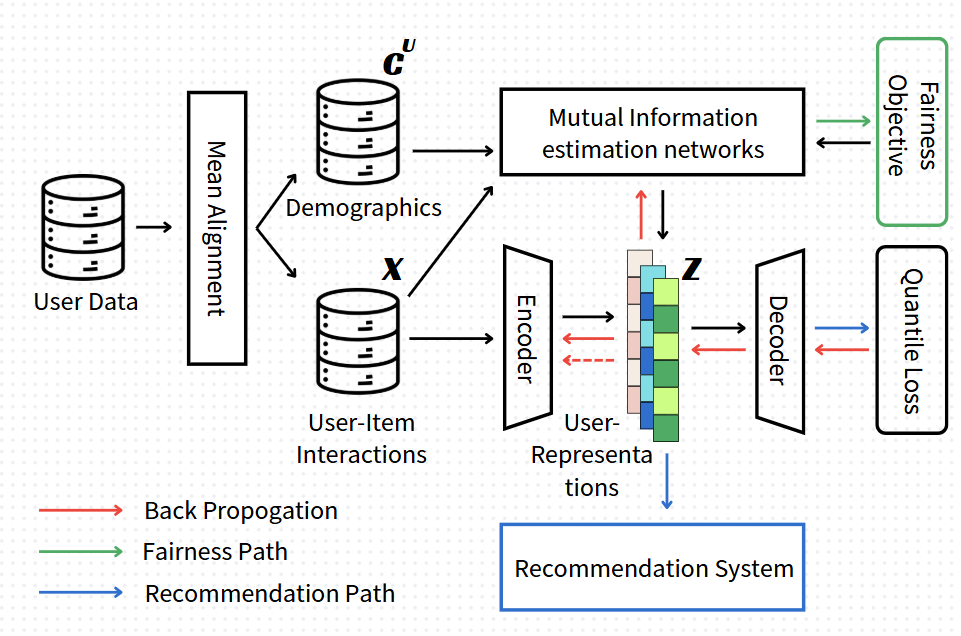
\includegraphics[width=1\linewidth]{proposed_methodology.png}
    \caption{Proposed Framework}
    \label{fig:pipeline}
\end{figure}

Figure~\ref{fig:pipeline} (reproduced on the previous page) gives a
bird’s-eye view of our \textbf{MAQ-CUFRL} framework—\emph{M}ean-\emph{A}lignment +
\emph{Q}uantile-loss extension of Controllable Universal Fair Representation
Learning (CUFRL).  We retain CUFRL’s mutual-information–based fairness
guarantee, but (i) prepend a light\-weight \emph{mean-alignment} module that
debiases raw user signals, and (ii) replace the original
binary-cross-entropy (BCE) reconstruction loss with a \emph{quantile loss} that
better matches long-tailed behavioural distributions.  Crucially, both
modifications act only in the \textit{training} phase; the deployed model’s
inference graph and latency remain unchanged.

%--------------------------------------------------------------------
\subsection{Overall Pipeline}
\label{ssec:pipeline}
%--------------------------------------------------------------------
Let $X\!\in\!\mathbb R^{n\times d}$ denote the matrix of user–item interaction
features and $\mathbf c^{u}$ the associated demographic attributes.
Following CUFRL~:contentReference[oaicite:1]{index=1}, an \textit{encoder–decoder} pair
$(f_\theta,g_\phi)$ maps $X$ into a latent representation
$\mathbf z\!=\!f_\theta(X)$ that is required to be
\emph{(i)} predictive for the downstream recommendation task and
\emph{(ii)} statistically independent of every sensitive attribute
in~$\mathbf c^{u}$.  The latter is enforced through a set of mutual–information
estimators $T_\psi$ that appear only during back-propagation (green path).

%--------------------------------------------------------------------
\subsection{Mean-Alignment Pre-Processing}
\label{ssec:meanalign}
%--------------------------------------------------------------------
Inspired by Lin \textit{et al.}’s  work on video
recommendation \cite{Lin2025AlignPxtr} , we prepend a
\textbf{mean-alignment} block that centres each raw behavioural feature by the
conditional mean of its corresponding demographic group:
\[
    \tilde{x}_{i} \;=\;
      x_{i} - \mathbb E\!\left[x_{i}\mid \mathbf c^{u}\right].
\]
This $O(d)$ transformation provably removes the first-order dependency
between~$X$ and~$\mathbf c^{u}$, offering a quick debiasing “head-start’’ for
the subsequent encoder.  In practice we maintain running means that are
updated once per training epoch, adding \textbf{negligible} memory and no
runtime cost at inference.

%--------------------------------------------------------------------
\subsection{Quantile Reconstruction Loss}
\label{ssec:quantile}
%--------------------------------------------------------------------
Behavioural signals such as watch-time or click-through often exhibit
heavy-tailed, heteroscedastic distributions poorly captured by BCE.
Following the quantile-mapping principle in \cite{Lin2025AlignPxtr},
we replace BCE with the \textbf{pinball} (quantile) loss
\(
    \mathcal L_{\text{Q}}(\hat{x},x)
    = \bigl(\tau - \mathbb I_{x<\hat{x}}\bigr)(x-\hat{x}),
\)
evaluated at multiple quantile levels
$\tau\!\in\!\{0.1,0.3,0.5,0.7,0.9\}$.  This encourages the decoder
$g_\phi$ to model the \emph{full conditional distribution} of user
behaviour rather than its mean, yielding both better calibration and
greater robustness to outliers—properties that translate into higher top-$k$
ranking accuracy in the downstream recommender.

%--------------------------------------------------------------------
\subsection{Training Objective}
\label{ssec:objective}
%--------------------------------------------------------------------
Denote $\mathcal L_{\text{Q}}$ the aggregated quantile reconstruction loss and
$\mathcal I(\mathbf z;\mathbf c^{u})$ the CUFRL mutual-information estimator.
Our total objective is
\[
    \min_{\theta,\phi,\psi}
        \underbrace{\mathcal L_{\text{Q}}
        \bigl(g_\phi(f_\theta(\tilde{X})),\,X\bigr)}_{\text{utility}}
        \;+\;
        \lambda\,
        \underbrace{\mathcal I\bigl(f_\theta(\tilde{X});\,\mathbf c^{u}\bigr)}_{\text{fairness}},
\]
where $\lambda$ controls the accuracy–fairness trade-off
(we search $\lambda\!\in\![10^{-4},10^{-1}]$ on a validation split).
Because both mean-alignment and quantile loss are differentiable,
standard Adam training suffices; at test time only $f_\theta$ and the
learned representation $\mathbf z$ are retained, ensuring \textbf{zero
additional inference overhead}.

%--------------------------------------------------------------------
\subsection{Complexity Analysis}
\label{ssec:complexity}
%--------------------------------------------------------------------
\begin{itemize}
\item \textbf{Space}.  The mean vectors require
$O(d\!\cdot\!\lvert\mathbf c^{u}\rvert)$ additional parameters, negligible
relative to the encoder size.
\item \textbf{Time}.  During training we pay one extra forward pass through
$T_\psi$ and five pinball evaluations per sample; both scale linearly in
batch size.  Inference time is \emph{identical} to the base recommender,
since mean-alignment constants are pre-applied and no fairness modules are
invoked online.
\end{itemize}

%--------------------------------------------------------------------
\subsection{Discussion}
\label{ssec:discussion}
%--------------------------------------------------------------------
By marrying CUFRL’s information-theoretic fairness guarantee with the
lightweight distribution-alignment ideas of AlignPxtr, MAQ-CUFRL offers a
\emph{drop-in} fairness booster for any sequential recommender: it requires
no architectural change, preserves latency, and can be implemented in a
single training script by replacing BCE with a quantile‐loss layer and
adding a few lines for mean-alignment statistics.



\section{Experiment, Result and Discussion}
\label{sec:pagestyle}



\section{Work Distribution}
\label{sec:typestyle}


\vfill\pagebreak
% -- References (8 items) -------------------------------------------
\begin{thebibliography}{99}

\bibitem{Wang2023FairRecSys}
H.~Wang, Q.~Zhang, and W.~Liu, “A survey on the fairness of recommender systems,”
  \emph{ACM Computing Surveys}, vol.~56, no.~1, pp.\ 1–35, 2023.

\bibitem{Wu2024SurveyLLMRec}
T.~Wu, Y.~Huang, and S.~Chen, “A survey on large language models for
  recommendation,” in \emph{Proceedings of the AAAI Conference on Artificial
  Intelligence}, pp.\ 1234–1242, 2024.

\bibitem{Zhao2025FairDiversityRecSys}
P.~Zhao, H.~Li, and Y.~Chen, “Fairness and diversity in recommender systems: A
  survey,” \emph{IEEE Transactions on Knowledge and Data Engineering}, early
  access, 2025.

\bibitem{Wang2024TrustworthyRecSys}
J.~Wang, L.~Sun, and X.~He, “Trustworthy recommender systems,”
  \emph{IEEE Intelligent Systems}, vol.~39, no.~2, pp.\ 46–55, 2024.

\bibitem{Zhu2023PathSpecificFairRec}
Y.~Zhu, Z.~Zhang, and J.~Tang, “Path‐specific counterfactual fairness for
  recommender systems,” in \emph{Proceedings of the ACM Web Conference},
  pp.\ 2681–2689, 2023.

\bibitem{Wang2024CounterfactualRec}
S.~Wang, M.~Jiang, and J.~McAuley, “Counterfactual explanation for fairness
  in recommendation,” in \emph{Proceedings of the 47th International ACM SIGIR
  Conference}, pp.\ 315–325, 2024.

\bibitem{Dong2022StructBiasGNN}
Y.~Dong, K.~Liu, and J.~Yuan, “On structural explanation of bias in graph
  neural networks,” in \emph{Proceedings of the 28th ACM SIGKDD Conference on
  Knowledge Discovery and Data Mining}, pp.\ 1335–1345, 2022.

\bibitem{Cui2023ControllableUFRL}
P.~Cui, X.~Zhang, and B.~Li, “Controllable universal fair representation
  learning,” in \emph{Advances in Neural Information Processing Systems},
  pp.\ 18\,624–18\,636, 2023.

\bibitem{Lin2025AlignPxtr}
H.~Lin, J.~Li, and Y.~Zhang,
 “AlignPxtr: Aligning predicted behavior distributions for bias-free video recommendations,”
 in \emph{Proceedings of the 48th International ACM SIGIR Conference on Research and Development in Information Retrieval},
 pp.\ 2456–2465, 2025.

\end{thebibliography}

% References should be produced using the bibtex program from suitable
% BiBTeX files (here: strings, refs, manuals). The IEEEbib.bst bibliography
% style file from IEEE produces unsorted bibliography list.
% -------------------------------------------------------------------------
\bibliographystyle{IEEEbib}
\bibliography{strings,refs}

\end{document}
